\documentclass[main.tex]{subfiles}

\begin{document}

\begin{definition}
We adopt the following notations
\begin{itemize}
\item $\mathcal H=\mathcal H^+=\{\operatorname{Im}(z)>0\}$ is the upper half plane
\item $\mathcal H^-=\{\operatorname{Im}(z)<0\}$ is lower half plane
\item $\mathcal H^\pm=\mathcal H^+\cup\mathcal H^-$
\item $\mathbb P^1(\mathbb C)=\{[z_0,z_1]\}$ is the complex projective line
\item $\mathbb CP^1$ is the Riemann sphere $\mathbb C\cup\{\infty\}$, $\mathbb RP^1=\mathbb R\cup\{\infty\}$
\item $\mathbb D$ is the unit disc
\end{itemize}
\end{definition}

\begin{remark}\hfill
\begin{itemize}
\item $\PSL_2(\mathbb R)=\SL_2(\mathbb R)/Z=\GL^+_2(\mathbb R)/Z\leq\GL_2(\mathbb R)/Z=\PGL_2(\mathbb R)$ is a subgroup of index $2$, $\PGL_2(\mathbb R)$ has two connected components, $\PSL_2(\mathbb R)$ is its identity component
\item $\PSL_2(\mathbb C)=\SL_2(\mathbb C)/Z=\GL_2(\mathbb C)/Z=\PGL_2(\mathbb C)$
\end{itemize}
\end{remark}

\begin{definition}
Consider
\[\mathbb C^2-\{0\}\to\mathbb CP^1,\quad\begin{bmatrix}
z_0 \\
z_1
\end{bmatrix}\mapsto\dfrac{z_0}{z_1}\]
then the action of $\GL_2(\mathbb C)$ on $\mathbb C^2-\{0\}$ by matrix multiplication
\[
\begin{bmatrix}
a&b \\
c&d
\end{bmatrix}\begin{bmatrix}
z_0 \\
z_1
\end{bmatrix}=\begin{bmatrix}
az_0+bz_1 \\
cz_0+dz_1
\end{bmatrix}
\]
induces an action on $\mathbb P^1(\mathbb C)\cong\mathbb CP^1$ by \textit{fractional linear transformation}
\[
\begin{bmatrix}
a&b \\
c&d
\end{bmatrix}z=\frac{az+b}{cz+d}
\]
Since scalar matrices act trivially, this induces an action of $\PGL_2(\mathbb C)$ on $\mathbb CP^1$
\end{definition}

\begin{fact}\hfill
\begin{enumerate}
\item Under this action, $\PGL_2(\mathbb C)$ is identified with the holomorphic automorphism group of $\mathbb CP^1$, also the algebraic automorphism group of $\mathbb P^1(\mathbb C)$
\item For any three distinct points $z_1,z_2,z_3\in\mathbb CP^1$, there exists a unique $g\in\PGL_2(\mathbb C)$ such that $gz_1=0$, $gz_2=1$, $gz_3=\infty$. So any non-scalar matrix has at most two fixed points on $\mathbb CP^1$
\end{enumerate}
\end{fact}

\begin{lemma}\hfill
\begin{enumerate}
\item $\PSL_2(\mathbb R)$ has three orbits on $\mathbb CP^1$: $\mathcal H,\mathcal H^-,\mathbb RP^1$
\item $\PGL_2(\mathbb R)$ has two orbits on $\mathbb CP^1$: $\mathcal H^\pm,\mathbb RP^1$
\item $\PSL_2(\mathbb R)$ is the group of holomorphic automorphisms of $\mathcal H$
\end{enumerate}
\end{lemma}

\begin{proof}
If $g=\begin{bmatrix}
a&b\\
c&d
\end{bmatrix}\in \GL_2(\mathbb R)$, then
\begin{align*}
\operatorname{Im}(gz)=\operatorname{Im}\frac{(az+b)(c\bar z+d)}{|cz+d|^2}=\operatorname{Im}\frac{ac|z|^2+adz+bc\bar z+bd}{|cz+d|^2}=\frac{(ad-bc)\operatorname{Im}z}{|cz+d|^2} =\frac{\det(g)}{|cz+d|^2}\operatorname{Im}z
\end{align*}
So $\PSL_2(\mathbb R)$ preserves $\mathcal H,\mathcal H^-,\mathbb{RP}^1$. While $\begin{bmatrix}
1&0 \\
0&-1
\end{bmatrix}\in\PGL_2(\mathbb R)$ interchanges $\mathcal H$, $\mathcal H^-$. $\PSL_2(\mathbb R)$ acts transitively on $\mathcal H$ since for any $(x,y)\in\mathcal H$
\[\begin{bmatrix}
y^{\frac{1}{2}}&xy^{-\frac{1}{2}} \\
0&y^{-\frac{1}{2}}
\end{bmatrix}\cdot i=x+yi\]
For 3. first use Cayley transformation $\begin{bmatrix}
1&-i\\
1&i
\end{bmatrix}$ which induces an isomorphism $\mathcal H\to\mathbb D$, then use Schwartz lemma to determine $\Aut(\mathbb D)$, and then translate back to $\mathcal H$
\end{proof}

\begin{exercise}
The stabilizer of $i$ in $\SL_2(\mathbb R)$ is
\[\SO_2(\mathbb R)=\left\{\begin{bmatrix}
\cos\theta&\sin\theta \\
-\sin\theta&\cos\theta
\end{bmatrix}\middle|\theta\in\mathbb R\right\}\]
So the stabilier of $i$ in $\PSL_2(\mathbb R)$ is $\SO_2(\mathbb R)/\{\pm I\}\cong\operatorname{PSO}_2(\mathbb R)$. And therefore $\mathcal H\cong \SL_2(\mathbb R)/\SO_2(\mathbb R)\cong\PSL_2(\mathbb R)/\operatorname{PSO}_2(\mathbb R)$ is a homogeneous space
\end{exercise}

\begin{exercise}
For $g\in\SL_2(\mathbb R)$
\[
g^*dz=d(gz)=d\left(\frac{az+b}{cz+d}\right)=\frac{dz}{(cz+d)^2}
\]
So we have
\[
g^*(dx^2+dy^2)=g^*(dzd\bar z)=\frac{dzd\bar z}{(cz+d)^2(c\bar z+d)^2}=|cz+d|^{-4}(dx^2+dy^2)
\]
Hence
\[
g^*(y^{-2}(dx^2+dy^2))=(y\circ g)^2g^*(dx^2+dy^2)=\operatorname{Im}(gz)^{-2}|cz+d|^{-4}(dx^2+dy^2)=y^{-2}(dx^2+dy^2)
\]
\end{exercise}

\begin{definition}
Define the \textit{hyperbolic metric} on $\mathcal H$ to be $\dfrac{dx^2+dy^2}{y^2}$. Then $\mathcal H$ becomes a model of hyperbolic plane: a two dimensional simply connected Riemannian manifold with constant Gaussian curvature $-1$
\end{definition}

\begin{proposition}
$\PSL_2(\mathbb R)=\Isom^+(\mathcal H)$, the group of orientation preserving isometries. The group of isometries $\Isom(\mathcal H)$ is genenrated by $\Isom^+(\mathcal H)$ and reflection $z\mapsto-\bar z$
\end{proposition}

\begin{proof}
We have already seen $\PSL_2(\mathbb R)=\Hol(\mathcal H)$, the group of holomorphic automorphisms and $\PSL_2(\mathbb R)\leq\Isom^+(\mathcal H)$, but $\Isom^+(\mathcal H)\leq\Hol(\mathcal H)$ since orientation preserving conformal maps are holomorphic
\end{proof}

\begin{fact}
The geodesics on $\mathcal H$ are semi-circles othogonal to the real axis and half-lines orthogonal to the real axis, see [Miyake, Lemma 1.4.1]
\begin{center}
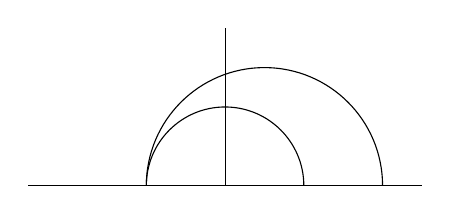
\begin{tikzpicture}
\draw (-2.5,0)--(2.5,0);
\draw (0,0)--(0,2);
\draw (1,0) arc (0:180:1);
\draw (2,0) arc (0:180:1.5);
\end{tikzpicture}
\end{center}
The hyperbolic metric induces a volume form $d\mu=\dfrac{dx\wedge dy}{y^2}$, and the hyperbolic Laplace operator $\Delta=-y^{-2}\left(\dfrac{\partial^2}{\partial x^2}+\dfrac{\partial^2}{\partial y^2}\right)$
\end{fact}

\begin{exercise}
 $d\mu,\Delta$ are invariant under $\PSL_2(\mathbb R)$ action (since the action preserves the metric)
\end{exercise}

\begin{theorem}[Classification of motions]
$g=\begin{bmatrix}
a&b\\
c&d
\end{bmatrix}\in\SL_2(\mathbb R)$ and $g\neq\pm I$, then $g$ has one or two fixed points on $\mathbb {CP}^1$
\end{theorem}

\begin{proof}
\begin{enumerate}[leftmargin=*, label=Case \arabic*:]
\item $c=0$
\begin{enumerate}[leftmargin=*, label=case \roman*:]
\item $a=d=\pm1$, so $b\neq0$, $g$ is a translation on $\mathbb{CP}^1$, $\infty$ is the only fixed point
\item $a\neq d$, $g$ is a linear function on $\mathbb{CP}^1$, $\infty,\dfrac{b}{d-a}\in\mathbb R$ are the two fixed points
\end{enumerate}
\item $c\neq0$, then $\infty\mapsto\dfrac{a}{c}$ is not fixed
\[\frac{az+b}{cz+d}=z\Rightarrow z=\frac{(a-d)\pm\sqrt{(a+d)^2-4}}{2c}\]
\begin{enumerate}[leftmargin=*, label=case \roman*:]
\item $|a+d|=2$, the only one fixed point is $\dfrac{a-d}{2c}\in\mathbb R$
\item $|a+d|>2$, there are two fixed points
\item $|a+d|<2$, there are two fixed points in $\mathcal H,\mathcal H^-$ and are conjugate of each other
\end{enumerate}
\end{enumerate}
In summary, there are three kinds of non-identity fractional linear transformation
\begin{enumerate}
\item Parabolic: When $|\tr g|=2$, only one fixed point, which is on $\mathbb {RP}^1$
\item Hyperbolic: When $|\tr g|>2$, two fixed points, both in $\mathbb{RP}^1$
\item Elliptic: When $|\tr g|<2$, two fixed points, one in $\mathcal H$, the other one in $\mathcal H^-$
\end{enumerate}
\end{proof}

\begin{example}
Translation $\begin{bmatrix}
1&b\\
0&1
\end{bmatrix}:z\mapsto z+b$ is a parabolic motion. In general, parabolic elements move points along \textit{horocycles}\index{Horocycle}, i.e. horiontal lines or circles tangent to the $x$-axis
\begin{center}
\begin{tikzpicture}
\draw[->](-4,0)--(4,0);
\draw[->](0,-1)--(0,3);
\foreach \i in {-4,-2,...,0}
{
\draw[->] (\i,2.5)--(\i+2,2.5);
}
\draw(2,2.5)--(4,2.5);
\foreach \x/\a/\b in {(-1,1)/180/90,(0,2)/90/0,(1,1)/0/-90,(0,0)/-90/-180}
{
\draw[->] \x arc (\a:\b:1);
}
\end{tikzpicture}
\end{center}
One can view horocycles as circles in $\mathbb{CP}^1=S^2$ that are tangent to $\mathbb{RP}^1=S^1$.
\textcolor{blue}{
$\PSL_2(\mathbb R)$ action takes horocycles to horocycles and acts transitiviely on the set of horocycles. For any horizontal horocycle (say $\operatorname{Im}z=1$), its stabilizer is $U=\left\{\begin{bmatrix}
1&*\\
0&1
\end{bmatrix}\right\}$, identified with its image in $\PSL_2(\mathbb R)$. Hence the set of horocycles can be identified with $\PSL_2(\mathbb R)/U\cong(\mathbb R^2-\{0\})/\{\pm I\}$ (note that $SL_2(\mathbb R)/U\cong\mathbb R^2-\{0\}$)
}
\end{example}

\begin{example}
$g=\begin{bmatrix}
a&0 \\
0&a^{-1}
\end{bmatrix}:z\mapsto a^2z$ is a hyperbolic motion, fixing $0,\infty$. In general, hyperbolic element moves points along \textit{hypercycles}\index{Hypercycle}, i.e. intersections of circles in $\mathbb{CP}^1$ passing through the fixed points on $\mathbb {RP}^1$ with $\mathcal H$
\begin{center}
\begin{tikzpicture}[yscale=0.5]
\draw (-4,0)--(4,0);
\node at (4,0) [right] {$\mathbb{RP}^1$};
\node at (-3,0) [below] {repelling};
\node at (3,0) [below] {attracting};
\draw[->-=.5] (-3,0) to [curve through ={(0,1)}] (3,0) ;
\draw[->-=.5] (-3,0) to [curve through ={(0,2)}] (3,0) ;
\draw[->-=.5] (-3,0) to [curve through ={(0,3)}] (3,0) ;
\end{tikzpicture}
\end{center}
\end{example}

\begin{example}
$g=\begin{bmatrix}
\cos\theta&\sin\theta \\
-\sin\theta&\cos\theta
\end{bmatrix}$ is a elliptic motion, moving points along circles with \textit{hyperbolic center} $i$, fixes $i$, induces counter-clockwise rotation of angle $2\theta$ on the tangent space at $i$
\begin{center}
\begin{tikzpicture}
\draw[->] (-4,0)--(4,0);
\draw[->] (0,-1)--(0,4.5);
\draw[->-=.5] (0,0.5) arc (-90:90:0.75);\draw[->-=.5] (0,2) arc (90:270:0.75);
\draw[->-=.5] (0,{1/3}) arc (-90:90:{(3-0.3333333333)/2});\draw[->-=.5] (0,3) arc (90:270:{(3-0.3333333333)/2});
\draw[->-=.5] (0,0.25) arc (-90:90:{(4-0.25)/2});\draw[->-=.5] (0,4) arc (90:270:{(4-0.25)/2});
\filldraw (0,1) circle (0.02);
\node at (0,1) [right] {$i$};
\end{tikzpicture}
\end{center}
\end{example}

\begin{remark}
Elliptic motions may have finite order ($\theta=\frac{\pi}{n},n\in\mathbb Z$), parabolic and hyperbolic motions have infinite orders
\end{remark}

\end{document}